% Created by tikzDevice version 0.10.1 on 2016-08-26 09:59:53
% !TEX encoding = UTF-8 Unicode
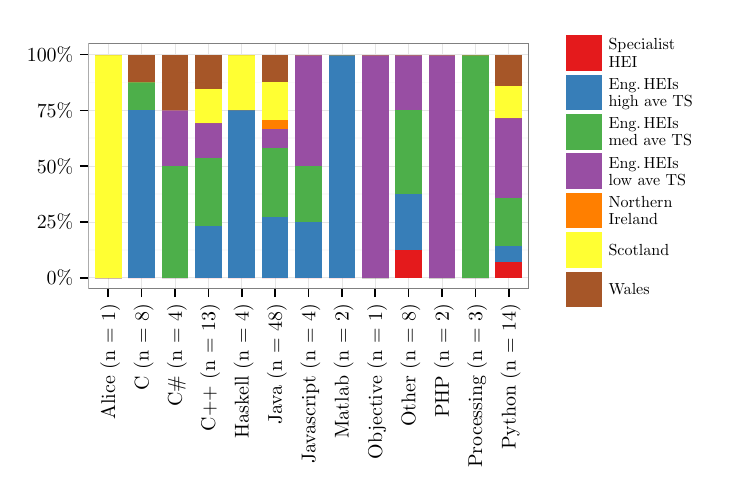
\begin{tikzpicture}[x=1pt,y=1pt]
\definecolor{fillColor}{RGB}{255,255,255}
\path[use as bounding box,fill=fillColor,fill opacity=0.00] (0,0) rectangle (252.94,158.99);
\begin{scope}
\path[clip] (  0.00,  0.00) rectangle (252.94,158.99);
\definecolor{drawColor}{RGB}{255,255,255}
\definecolor{fillColor}{RGB}{255,255,255}

\path[draw=drawColor,line width= 0.6pt,line join=round,line cap=round,fill=fillColor] (  0.00,  0.00) rectangle (252.94,158.99);
\end{scope}
\begin{scope}
\path[clip] ( 21.89, 64.59) rectangle (181.07,153.30);
\definecolor{fillColor}{RGB}{255,255,255}

\path[fill=fillColor] ( 21.89, 64.59) rectangle (181.07,153.30);
\definecolor{drawColor}{gray}{0.98}

\path[draw=drawColor,line width= 0.6pt,line join=round] ( 21.89, 78.70) --
	(181.07, 78.70);

\path[draw=drawColor,line width= 0.6pt,line join=round] ( 21.89, 98.86) --
	(181.07, 98.86);

\path[draw=drawColor,line width= 0.6pt,line join=round] ( 21.89,119.03) --
	(181.07,119.03);

\path[draw=drawColor,line width= 0.6pt,line join=round] ( 21.89,139.19) --
	(181.07,139.19);
\definecolor{drawColor}{gray}{0.90}

\path[draw=drawColor,line width= 0.2pt,line join=round] ( 21.89, 68.62) --
	(181.07, 68.62);

\path[draw=drawColor,line width= 0.2pt,line join=round] ( 21.89, 88.78) --
	(181.07, 88.78);

\path[draw=drawColor,line width= 0.2pt,line join=round] ( 21.89,108.94) --
	(181.07,108.94);

\path[draw=drawColor,line width= 0.2pt,line join=round] ( 21.89,129.11) --
	(181.07,129.11);

\path[draw=drawColor,line width= 0.2pt,line join=round] ( 21.89,149.27) --
	(181.07,149.27);

\path[draw=drawColor,line width= 0.2pt,line join=round] ( 29.12, 64.59) --
	( 29.12,153.30);

\path[draw=drawColor,line width= 0.2pt,line join=round] ( 41.18, 64.59) --
	( 41.18,153.30);

\path[draw=drawColor,line width= 0.2pt,line join=round] ( 53.24, 64.59) --
	( 53.24,153.30);

\path[draw=drawColor,line width= 0.2pt,line join=round] ( 65.30, 64.59) --
	( 65.30,153.30);

\path[draw=drawColor,line width= 0.2pt,line join=round] ( 77.36, 64.59) --
	( 77.36,153.30);

\path[draw=drawColor,line width= 0.2pt,line join=round] ( 89.42, 64.59) --
	( 89.42,153.30);

\path[draw=drawColor,line width= 0.2pt,line join=round] (101.48, 64.59) --
	(101.48,153.30);

\path[draw=drawColor,line width= 0.2pt,line join=round] (113.54, 64.59) --
	(113.54,153.30);

\path[draw=drawColor,line width= 0.2pt,line join=round] (125.60, 64.59) --
	(125.60,153.30);

\path[draw=drawColor,line width= 0.2pt,line join=round] (137.66, 64.59) --
	(137.66,153.30);

\path[draw=drawColor,line width= 0.2pt,line join=round] (149.72, 64.59) --
	(149.72,153.30);

\path[draw=drawColor,line width= 0.2pt,line join=round] (161.78, 64.59) --
	(161.78,153.30);

\path[draw=drawColor,line width= 0.2pt,line join=round] (173.84, 64.59) --
	(173.84,153.30);
\definecolor{fillColor}{RGB}{228,26,28}

\path[fill=fillColor] ( 24.30, 68.62) rectangle ( 33.95, 68.62);
\definecolor{fillColor}{RGB}{55,126,184}

\path[fill=fillColor] ( 24.30, 68.62) rectangle ( 33.95, 68.62);
\definecolor{fillColor}{RGB}{77,175,74}

\path[fill=fillColor] ( 24.30, 68.62) rectangle ( 33.95, 68.62);
\definecolor{fillColor}{RGB}{152,78,163}

\path[fill=fillColor] ( 24.30, 68.62) rectangle ( 33.95, 68.62);
\definecolor{fillColor}{RGB}{255,127,0}

\path[fill=fillColor] ( 24.30, 68.62) rectangle ( 33.95, 68.62);
\definecolor{fillColor}{RGB}{255,255,51}

\path[fill=fillColor] ( 24.30, 68.62) rectangle ( 33.95,149.27);
\definecolor{fillColor}{RGB}{166,86,40}

\path[fill=fillColor] ( 24.30,149.27) rectangle ( 33.95,149.27);
\definecolor{fillColor}{RGB}{228,26,28}

\path[fill=fillColor] ( 36.36, 68.62) rectangle ( 46.01, 68.62);
\definecolor{fillColor}{RGB}{55,126,184}

\path[fill=fillColor] ( 36.36, 68.62) rectangle ( 46.01,129.11);
\definecolor{fillColor}{RGB}{77,175,74}

\path[fill=fillColor] ( 36.36,129.11) rectangle ( 46.01,139.19);
\definecolor{fillColor}{RGB}{152,78,163}

\path[fill=fillColor] ( 36.36,139.19) rectangle ( 46.01,139.19);
\definecolor{fillColor}{RGB}{255,127,0}

\path[fill=fillColor] ( 36.36,139.19) rectangle ( 46.01,139.19);
\definecolor{fillColor}{RGB}{255,255,51}

\path[fill=fillColor] ( 36.36,139.19) rectangle ( 46.01,139.19);
\definecolor{fillColor}{RGB}{166,86,40}

\path[fill=fillColor] ( 36.36,139.19) rectangle ( 46.01,149.27);
\definecolor{fillColor}{RGB}{228,26,28}

\path[fill=fillColor] ( 48.42, 68.62) rectangle ( 58.07, 68.62);
\definecolor{fillColor}{RGB}{55,126,184}

\path[fill=fillColor] ( 48.42, 68.62) rectangle ( 58.07, 68.62);
\definecolor{fillColor}{RGB}{77,175,74}

\path[fill=fillColor] ( 48.42, 68.62) rectangle ( 58.07,108.94);
\definecolor{fillColor}{RGB}{152,78,163}

\path[fill=fillColor] ( 48.42,108.94) rectangle ( 58.07,129.11);
\definecolor{fillColor}{RGB}{255,127,0}

\path[fill=fillColor] ( 48.42,129.11) rectangle ( 58.07,129.11);
\definecolor{fillColor}{RGB}{255,255,51}

\path[fill=fillColor] ( 48.42,129.11) rectangle ( 58.07,129.11);
\definecolor{fillColor}{RGB}{166,86,40}

\path[fill=fillColor] ( 48.42,129.11) rectangle ( 58.07,149.27);
\definecolor{fillColor}{RGB}{228,26,28}

\path[fill=fillColor] ( 60.48, 68.62) rectangle ( 70.13, 68.62);
\definecolor{fillColor}{RGB}{55,126,184}

\path[fill=fillColor] ( 60.48, 68.62) rectangle ( 70.13, 87.23);
\definecolor{fillColor}{RGB}{77,175,74}

\path[fill=fillColor] ( 60.48, 87.23) rectangle ( 70.13,112.05);
\definecolor{fillColor}{RGB}{152,78,163}

\path[fill=fillColor] ( 60.48,112.05) rectangle ( 70.13,124.45);
\definecolor{fillColor}{RGB}{255,127,0}

\path[fill=fillColor] ( 60.48,124.45) rectangle ( 70.13,124.45);
\definecolor{fillColor}{RGB}{255,255,51}

\path[fill=fillColor] ( 60.48,124.45) rectangle ( 70.13,136.86);
\definecolor{fillColor}{RGB}{166,86,40}

\path[fill=fillColor] ( 60.48,136.86) rectangle ( 70.13,149.27);
\definecolor{fillColor}{RGB}{228,26,28}

\path[fill=fillColor] ( 72.54, 68.62) rectangle ( 82.18, 68.62);
\definecolor{fillColor}{RGB}{55,126,184}

\path[fill=fillColor] ( 72.54, 68.62) rectangle ( 82.18,129.11);
\definecolor{fillColor}{RGB}{77,175,74}

\path[fill=fillColor] ( 72.54,129.11) rectangle ( 82.18,129.11);
\definecolor{fillColor}{RGB}{152,78,163}

\path[fill=fillColor] ( 72.54,129.11) rectangle ( 82.18,129.11);
\definecolor{fillColor}{RGB}{255,127,0}

\path[fill=fillColor] ( 72.54,129.11) rectangle ( 82.18,129.11);
\definecolor{fillColor}{RGB}{255,255,51}

\path[fill=fillColor] ( 72.54,129.11) rectangle ( 82.18,149.27);
\definecolor{fillColor}{RGB}{166,86,40}

\path[fill=fillColor] ( 72.54,149.27) rectangle ( 82.18,149.27);
\definecolor{fillColor}{RGB}{228,26,28}

\path[fill=fillColor] ( 84.60, 68.62) rectangle ( 94.24, 68.62);
\definecolor{fillColor}{RGB}{55,126,184}

\path[fill=fillColor] ( 84.60, 68.62) rectangle ( 94.24, 90.46);
\definecolor{fillColor}{RGB}{77,175,74}

\path[fill=fillColor] ( 84.60, 90.46) rectangle ( 94.24,115.67);
\definecolor{fillColor}{RGB}{152,78,163}

\path[fill=fillColor] ( 84.60,115.67) rectangle ( 94.24,122.39);
\definecolor{fillColor}{RGB}{255,127,0}

\path[fill=fillColor] ( 84.60,122.39) rectangle ( 94.24,125.75);
\definecolor{fillColor}{RGB}{255,255,51}

\path[fill=fillColor] ( 84.60,125.75) rectangle ( 94.24,139.19);
\definecolor{fillColor}{RGB}{166,86,40}

\path[fill=fillColor] ( 84.60,139.19) rectangle ( 94.24,149.27);
\definecolor{fillColor}{RGB}{228,26,28}

\path[fill=fillColor] ( 96.66, 68.62) rectangle (106.30, 68.62);
\definecolor{fillColor}{RGB}{55,126,184}

\path[fill=fillColor] ( 96.66, 68.62) rectangle (106.30, 88.78);
\definecolor{fillColor}{RGB}{77,175,74}

\path[fill=fillColor] ( 96.66, 88.78) rectangle (106.30,108.94);
\definecolor{fillColor}{RGB}{152,78,163}

\path[fill=fillColor] ( 96.66,108.94) rectangle (106.30,149.27);
\definecolor{fillColor}{RGB}{255,127,0}

\path[fill=fillColor] ( 96.66,149.27) rectangle (106.30,149.27);
\definecolor{fillColor}{RGB}{255,255,51}

\path[fill=fillColor] ( 96.66,149.27) rectangle (106.30,149.27);
\definecolor{fillColor}{RGB}{166,86,40}

\path[fill=fillColor] ( 96.66,149.27) rectangle (106.30,149.27);
\definecolor{fillColor}{RGB}{228,26,28}

\path[fill=fillColor] (108.72, 68.62) rectangle (118.36, 68.62);
\definecolor{fillColor}{RGB}{55,126,184}

\path[fill=fillColor] (108.72, 68.62) rectangle (118.36,149.27);
\definecolor{fillColor}{RGB}{77,175,74}

\path[fill=fillColor] (108.72,149.27) rectangle (118.36,149.27);
\definecolor{fillColor}{RGB}{152,78,163}

\path[fill=fillColor] (108.72,149.27) rectangle (118.36,149.27);
\definecolor{fillColor}{RGB}{255,127,0}

\path[fill=fillColor] (108.72,149.27) rectangle (118.36,149.27);
\definecolor{fillColor}{RGB}{255,255,51}

\path[fill=fillColor] (108.72,149.27) rectangle (118.36,149.27);
\definecolor{fillColor}{RGB}{166,86,40}

\path[fill=fillColor] (108.72,149.27) rectangle (118.36,149.27);
\definecolor{fillColor}{RGB}{228,26,28}

\path[fill=fillColor] (120.77, 68.62) rectangle (130.42, 68.62);
\definecolor{fillColor}{RGB}{55,126,184}

\path[fill=fillColor] (120.77, 68.62) rectangle (130.42, 68.62);
\definecolor{fillColor}{RGB}{77,175,74}

\path[fill=fillColor] (120.77, 68.62) rectangle (130.42, 68.62);
\definecolor{fillColor}{RGB}{152,78,163}

\path[fill=fillColor] (120.77, 68.62) rectangle (130.42,149.27);
\definecolor{fillColor}{RGB}{255,127,0}

\path[fill=fillColor] (120.77,149.27) rectangle (130.42,149.27);
\definecolor{fillColor}{RGB}{255,255,51}

\path[fill=fillColor] (120.77,149.27) rectangle (130.42,149.27);
\definecolor{fillColor}{RGB}{166,86,40}

\path[fill=fillColor] (120.77,149.27) rectangle (130.42,149.27);
\definecolor{fillColor}{RGB}{228,26,28}

\path[fill=fillColor] (132.83, 68.62) rectangle (142.48, 78.70);
\definecolor{fillColor}{RGB}{55,126,184}

\path[fill=fillColor] (132.83, 78.70) rectangle (142.48, 98.86);
\definecolor{fillColor}{RGB}{77,175,74}

\path[fill=fillColor] (132.83, 98.86) rectangle (142.48,129.11);
\definecolor{fillColor}{RGB}{152,78,163}

\path[fill=fillColor] (132.83,129.11) rectangle (142.48,149.27);
\definecolor{fillColor}{RGB}{255,127,0}

\path[fill=fillColor] (132.83,149.27) rectangle (142.48,149.27);
\definecolor{fillColor}{RGB}{255,255,51}

\path[fill=fillColor] (132.83,149.27) rectangle (142.48,149.27);
\definecolor{fillColor}{RGB}{166,86,40}

\path[fill=fillColor] (132.83,149.27) rectangle (142.48,149.27);
\definecolor{fillColor}{RGB}{228,26,28}

\path[fill=fillColor] (144.89, 68.62) rectangle (154.54, 68.62);
\definecolor{fillColor}{RGB}{55,126,184}

\path[fill=fillColor] (144.89, 68.62) rectangle (154.54, 68.62);
\definecolor{fillColor}{RGB}{77,175,74}

\path[fill=fillColor] (144.89, 68.62) rectangle (154.54, 68.62);
\definecolor{fillColor}{RGB}{152,78,163}

\path[fill=fillColor] (144.89, 68.62) rectangle (154.54,149.27);
\definecolor{fillColor}{RGB}{255,127,0}

\path[fill=fillColor] (144.89,149.27) rectangle (154.54,149.27);
\definecolor{fillColor}{RGB}{255,255,51}

\path[fill=fillColor] (144.89,149.27) rectangle (154.54,149.27);
\definecolor{fillColor}{RGB}{166,86,40}

\path[fill=fillColor] (144.89,149.27) rectangle (154.54,149.27);
\definecolor{fillColor}{RGB}{228,26,28}

\path[fill=fillColor] (156.95, 68.62) rectangle (166.60, 68.62);
\definecolor{fillColor}{RGB}{55,126,184}

\path[fill=fillColor] (156.95, 68.62) rectangle (166.60, 68.62);
\definecolor{fillColor}{RGB}{77,175,74}

\path[fill=fillColor] (156.95, 68.62) rectangle (166.60,149.27);
\definecolor{fillColor}{RGB}{152,78,163}

\path[fill=fillColor] (156.95,149.27) rectangle (166.60,149.27);
\definecolor{fillColor}{RGB}{255,127,0}

\path[fill=fillColor] (156.95,149.27) rectangle (166.60,149.27);
\definecolor{fillColor}{RGB}{255,255,51}

\path[fill=fillColor] (156.95,149.27) rectangle (166.60,149.27);
\definecolor{fillColor}{RGB}{166,86,40}

\path[fill=fillColor] (156.95,149.27) rectangle (166.60,149.27);
\definecolor{fillColor}{RGB}{228,26,28}

\path[fill=fillColor] (169.01, 68.62) rectangle (178.66, 74.38);
\definecolor{fillColor}{RGB}{55,126,184}

\path[fill=fillColor] (169.01, 74.38) rectangle (178.66, 80.14);
\definecolor{fillColor}{RGB}{77,175,74}

\path[fill=fillColor] (169.01, 80.14) rectangle (178.66, 97.42);
\definecolor{fillColor}{RGB}{152,78,163}

\path[fill=fillColor] (169.01, 97.42) rectangle (178.66,126.23);
\definecolor{fillColor}{RGB}{255,127,0}

\path[fill=fillColor] (169.01,126.23) rectangle (178.66,126.23);
\definecolor{fillColor}{RGB}{255,255,51}

\path[fill=fillColor] (169.01,126.23) rectangle (178.66,137.75);
\definecolor{fillColor}{RGB}{166,86,40}

\path[fill=fillColor] (169.01,137.75) rectangle (178.66,149.27);
\definecolor{drawColor}{gray}{0.50}

\path[draw=drawColor,line width= 0.6pt,line join=round,line cap=round] ( 21.89, 64.59) rectangle (181.07,153.30);
\end{scope}
\begin{scope}
\path[clip] (  0.00,  0.00) rectangle (252.94,158.99);
\definecolor{drawColor}{RGB}{0,0,0}

\node[text=drawColor,anchor=base east,inner sep=0pt, outer sep=0pt, scale=  0.72] at ( 16.49, 66.14) {0\%};

\node[text=drawColor,anchor=base east,inner sep=0pt, outer sep=0pt, scale=  0.72] at ( 16.49, 86.30) {25\%};

\node[text=drawColor,anchor=base east,inner sep=0pt, outer sep=0pt, scale=  0.72] at ( 16.49,106.47) {50\%};

\node[text=drawColor,anchor=base east,inner sep=0pt, outer sep=0pt, scale=  0.72] at ( 16.49,126.63) {75\%};

\node[text=drawColor,anchor=base east,inner sep=0pt, outer sep=0pt, scale=  0.72] at ( 16.49,146.79) {100\%};
\end{scope}
\begin{scope}
\path[clip] (  0.00,  0.00) rectangle (252.94,158.99);
\definecolor{drawColor}{RGB}{0,0,0}

\path[draw=drawColor,line width= 0.6pt,line join=round] ( 18.89, 68.62) --
	( 21.89, 68.62);

\path[draw=drawColor,line width= 0.6pt,line join=round] ( 18.89, 88.78) --
	( 21.89, 88.78);

\path[draw=drawColor,line width= 0.6pt,line join=round] ( 18.89,108.94) --
	( 21.89,108.94);

\path[draw=drawColor,line width= 0.6pt,line join=round] ( 18.89,129.11) --
	( 21.89,129.11);

\path[draw=drawColor,line width= 0.6pt,line join=round] ( 18.89,149.27) --
	( 21.89,149.27);
\end{scope}
\begin{scope}
\path[clip] (  0.00,  0.00) rectangle (252.94,158.99);
\definecolor{drawColor}{RGB}{0,0,0}

\path[draw=drawColor,line width= 0.6pt,line join=round] ( 29.12, 61.59) --
	( 29.12, 64.59);

\path[draw=drawColor,line width= 0.6pt,line join=round] ( 41.18, 61.59) --
	( 41.18, 64.59);

\path[draw=drawColor,line width= 0.6pt,line join=round] ( 53.24, 61.59) --
	( 53.24, 64.59);

\path[draw=drawColor,line width= 0.6pt,line join=round] ( 65.30, 61.59) --
	( 65.30, 64.59);

\path[draw=drawColor,line width= 0.6pt,line join=round] ( 77.36, 61.59) --
	( 77.36, 64.59);

\path[draw=drawColor,line width= 0.6pt,line join=round] ( 89.42, 61.59) --
	( 89.42, 64.59);

\path[draw=drawColor,line width= 0.6pt,line join=round] (101.48, 61.59) --
	(101.48, 64.59);

\path[draw=drawColor,line width= 0.6pt,line join=round] (113.54, 61.59) --
	(113.54, 64.59);

\path[draw=drawColor,line width= 0.6pt,line join=round] (125.60, 61.59) --
	(125.60, 64.59);

\path[draw=drawColor,line width= 0.6pt,line join=round] (137.66, 61.59) --
	(137.66, 64.59);

\path[draw=drawColor,line width= 0.6pt,line join=round] (149.72, 61.59) --
	(149.72, 64.59);

\path[draw=drawColor,line width= 0.6pt,line join=round] (161.78, 61.59) --
	(161.78, 64.59);

\path[draw=drawColor,line width= 0.6pt,line join=round] (173.84, 61.59) --
	(173.84, 64.59);
\end{scope}
\begin{scope}
\path[clip] (  0.00,  0.00) rectangle (252.94,158.99);
\definecolor{drawColor}{RGB}{0,0,0}

\node[text=drawColor,rotate= 90.00,anchor=base east,inner sep=0pt, outer sep=0pt, scale=  0.72] at ( 31.60, 59.19) {Alice (n = 1)};

\node[text=drawColor,rotate= 90.00,anchor=base east,inner sep=0pt, outer sep=0pt, scale=  0.72] at ( 43.66, 59.19) {C (n = 8)};

\node[text=drawColor,rotate= 90.00,anchor=base east,inner sep=0pt, outer sep=0pt, scale=  0.72] at ( 55.72, 59.19) {C\# (n = 4)};

\node[text=drawColor,rotate= 90.00,anchor=base east,inner sep=0pt, outer sep=0pt, scale=  0.72] at ( 67.78, 59.19) {C++ (n = 13)};

\node[text=drawColor,rotate= 90.00,anchor=base east,inner sep=0pt, outer sep=0pt, scale=  0.72] at ( 79.84, 59.19) {Haskell (n = 4)};

\node[text=drawColor,rotate= 90.00,anchor=base east,inner sep=0pt, outer sep=0pt, scale=  0.72] at ( 91.90, 59.19) {Java (n = 48)};

\node[text=drawColor,rotate= 90.00,anchor=base east,inner sep=0pt, outer sep=0pt, scale=  0.72] at (103.96, 59.19) {Javascript (n = 4)};

\node[text=drawColor,rotate= 90.00,anchor=base east,inner sep=0pt, outer sep=0pt, scale=  0.72] at (116.02, 59.19) {Matlab (n = 2)};

\node[text=drawColor,rotate= 90.00,anchor=base east,inner sep=0pt, outer sep=0pt, scale=  0.72] at (128.08, 59.19) {Objective (n = 1)};

\node[text=drawColor,rotate= 90.00,anchor=base east,inner sep=0pt, outer sep=0pt, scale=  0.72] at (140.14, 59.19) {Other (n = 8)};

\node[text=drawColor,rotate= 90.00,anchor=base east,inner sep=0pt, outer sep=0pt, scale=  0.72] at (152.20, 59.19) {PHP (n = 2)};

\node[text=drawColor,rotate= 90.00,anchor=base east,inner sep=0pt, outer sep=0pt, scale=  0.72] at (164.26, 59.19) {Processing (n = 3)};

\node[text=drawColor,rotate= 90.00,anchor=base east,inner sep=0pt, outer sep=0pt, scale=  0.72] at (176.32, 59.19) {Python (n = 14)};
\end{scope}
\begin{scope}
\path[clip] (  0.00,  0.00) rectangle (252.94,158.99);
\definecolor{fillColor}{RGB}{255,255,255}

\path[fill=fillColor] (189.61, 53.08) rectangle (244.41,164.81);
\end{scope}
\begin{scope}
\path[clip] (  0.00,  0.00) rectangle (252.94,158.99);
\definecolor{fillColor}{RGB}{228,26,28}

\path[fill=fillColor] (194.59,143.42) rectangle (207.39,156.22);
\end{scope}
\begin{scope}
\path[clip] (  0.00,  0.00) rectangle (252.94,158.99);
\definecolor{fillColor}{RGB}{55,126,184}

\path[fill=fillColor] (194.59,129.19) rectangle (207.39,141.99);
\end{scope}
\begin{scope}
\path[clip] (  0.00,  0.00) rectangle (252.94,158.99);
\definecolor{fillColor}{RGB}{77,175,74}

\path[fill=fillColor] (194.59,114.96) rectangle (207.39,127.77);
\end{scope}
\begin{scope}
\path[clip] (  0.00,  0.00) rectangle (252.94,158.99);
\definecolor{fillColor}{RGB}{152,78,163}

\path[fill=fillColor] (194.59,100.74) rectangle (207.39,113.54);
\end{scope}
\begin{scope}
\path[clip] (  0.00,  0.00) rectangle (252.94,158.99);
\definecolor{fillColor}{RGB}{255,127,0}

\path[fill=fillColor] (194.59, 86.51) rectangle (207.39, 99.31);
\end{scope}
\begin{scope}
\path[clip] (  0.00,  0.00) rectangle (252.94,158.99);
\definecolor{fillColor}{RGB}{255,255,51}

\path[fill=fillColor] (194.59, 72.28) rectangle (207.39, 85.09);
\end{scope}
\begin{scope}
\path[clip] (  0.00,  0.00) rectangle (252.94,158.99);
\definecolor{fillColor}{RGB}{166,86,40}

\path[fill=fillColor] (194.59, 58.06) rectangle (207.39, 70.86);
\end{scope}
\begin{scope}
\path[clip] (  0.00,  0.00) rectangle (252.94,158.99);
\definecolor{drawColor}{RGB}{0,0,0}

\node[text=drawColor,anchor=base west,inner sep=0pt, outer sep=0pt, scale=  0.58] at (209.91,150.94) {Specialist};

\node[text=drawColor,anchor=base west,inner sep=0pt, outer sep=0pt, scale=  0.58] at (209.91,144.72) {HEI};
\end{scope}
\begin{scope}
\path[clip] (  0.00,  0.00) rectangle (252.94,158.99);
\definecolor{drawColor}{RGB}{0,0,0}

\node[text=drawColor,anchor=base west,inner sep=0pt, outer sep=0pt, scale=  0.58] at (209.91,136.72) {Eng.\,HEIs};

\node[text=drawColor,anchor=base west,inner sep=0pt, outer sep=0pt, scale=  0.58] at (209.91,130.50) {high ave TS};
\end{scope}
\begin{scope}
\path[clip] (  0.00,  0.00) rectangle (252.94,158.99);
\definecolor{drawColor}{RGB}{0,0,0}

\node[text=drawColor,anchor=base west,inner sep=0pt, outer sep=0pt, scale=  0.58] at (209.91,122.49) {Eng.\,HEIs};

\node[text=drawColor,anchor=base west,inner sep=0pt, outer sep=0pt, scale=  0.58] at (209.91,116.27) {med ave TS};
\end{scope}
\begin{scope}
\path[clip] (  0.00,  0.00) rectangle (252.94,158.99);
\definecolor{drawColor}{RGB}{0,0,0}

\node[text=drawColor,anchor=base west,inner sep=0pt, outer sep=0pt, scale=  0.58] at (209.91,108.26) {Eng.\,HEIs};

\node[text=drawColor,anchor=base west,inner sep=0pt, outer sep=0pt, scale=  0.58] at (209.91,102.04) {low ave TS};
\end{scope}
\begin{scope}
\path[clip] (  0.00,  0.00) rectangle (252.94,158.99);
\definecolor{drawColor}{RGB}{0,0,0}

\node[text=drawColor,anchor=base west,inner sep=0pt, outer sep=0pt, scale=  0.58] at (209.91, 94.04) {Northern};

\node[text=drawColor,anchor=base west,inner sep=0pt, outer sep=0pt, scale=  0.58] at (209.91, 87.82) {Ireland};
\end{scope}
\begin{scope}
\path[clip] (  0.00,  0.00) rectangle (252.94,158.99);
\definecolor{drawColor}{RGB}{0,0,0}

\node[text=drawColor,anchor=base west,inner sep=0pt, outer sep=0pt, scale=  0.58] at (209.91, 76.70) {Scotland};
\end{scope}
\begin{scope}
\path[clip] (  0.00,  0.00) rectangle (252.94,158.99);
\definecolor{drawColor}{RGB}{0,0,0}

\node[text=drawColor,anchor=base west,inner sep=0pt, outer sep=0pt, scale=  0.58] at (209.91, 62.48) {Wales};
\end{scope}
\end{tikzpicture}
